\chapter{Introduction}

The android operating system, which is provided by Google, is predicted to continue to have a dramatic increase in the market with around 1.5 billion Android-based devices to be shipped by 2021 sta. It is currently leading the mobile OS market with over 80\verb+%+ market share compared to iOS, Windows, Blackberry, and Symbian OS as Figure \ref{fig:marketshare}. The availability of diverse Android markets such as Google Play, the official store, and third-party markets makes Android devices a popular target to not only legitimate developers, but also malware developers. Over one billion devices have been sold and more than 65 billion downloads have been made from Google Play. Android apps can be found in different categories, such as educational apps, gaming apps, social media apps, entertainment apps, banking apps, etc.

\begin{figure}[htbp]
    \centering
    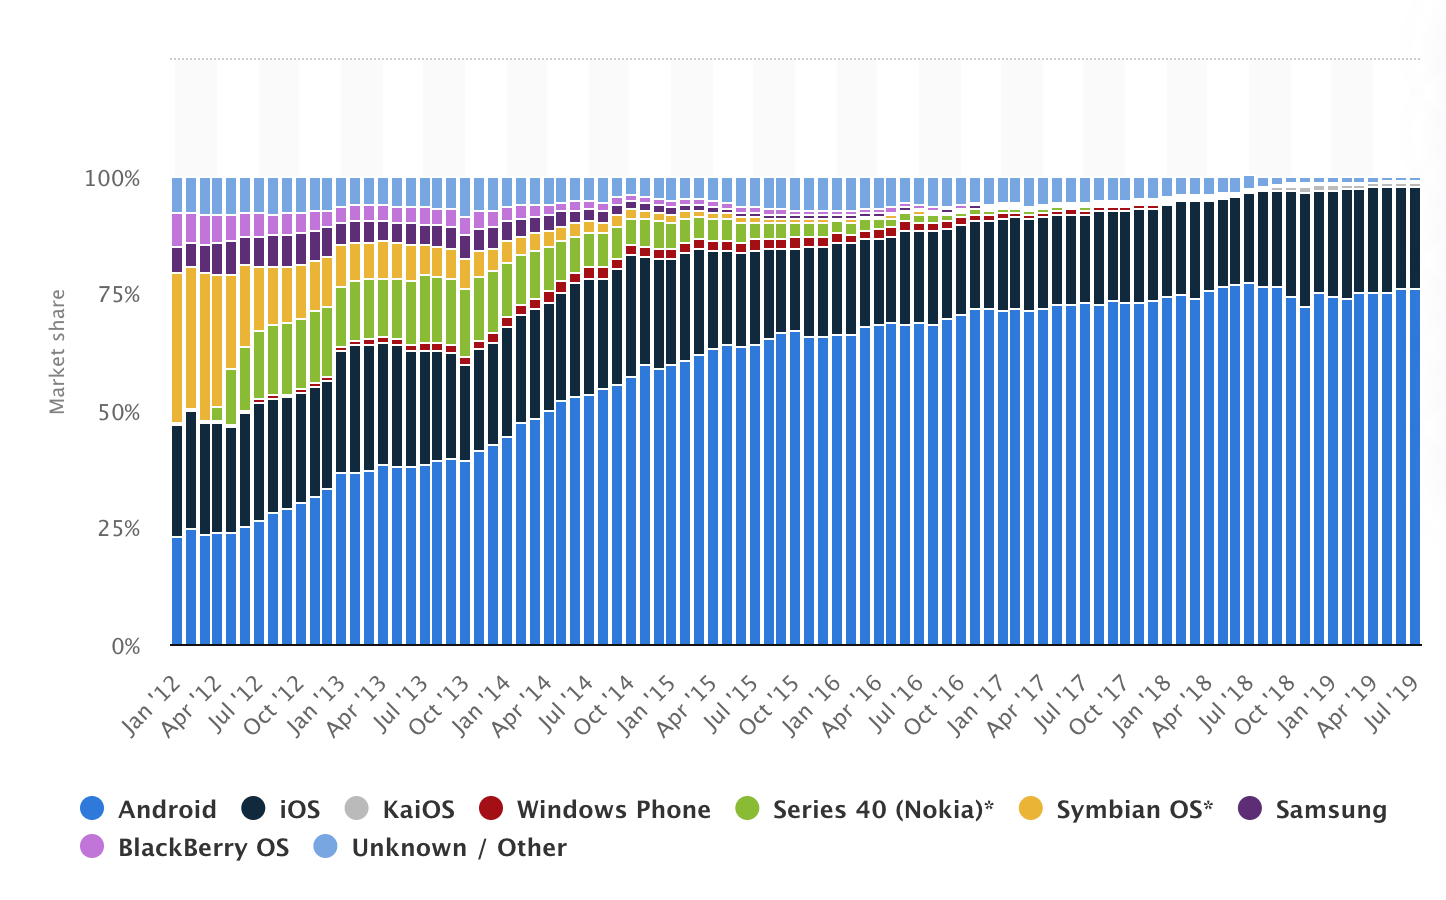
\includegraphics[scale=0.5]{./Figure/marketshare.png}
    \caption{Mobile operating systems's market share worldwide from January 2012 to July 2019 \cite{androidshare}}
    \label{fig:marketshare}
  \end{figure}

As a technology that is open source and widely adopted, Android is facing many challenges especially with malicious applications. The malware infected apps have the ability to send text messages to premium rate numbers without the user acknowledgment, gain access to private data, or even install code that can download and execute additional malware on the victim’s device. The malware can also be used to create mobile botnets \cite{dl-droid}. Over the last few years, the number of malware samples attacking Android has significantly increased as you can see at Figure \ref{fig:androidgraph}. Attacks on other connected things around the house gained momentum as well. While hidden apps and Adware remain by far the most common form of mobile threats in Android, the others are growing and learning how to infect other types of devices as well. According to a recent report from McAfee \cite{mcafee}, detections of backdoors,cryptomining, fake apps, and banking Trojans all
increased substantially in the latter half of the year. 

\begin{figure}[htbp]
    \centering
    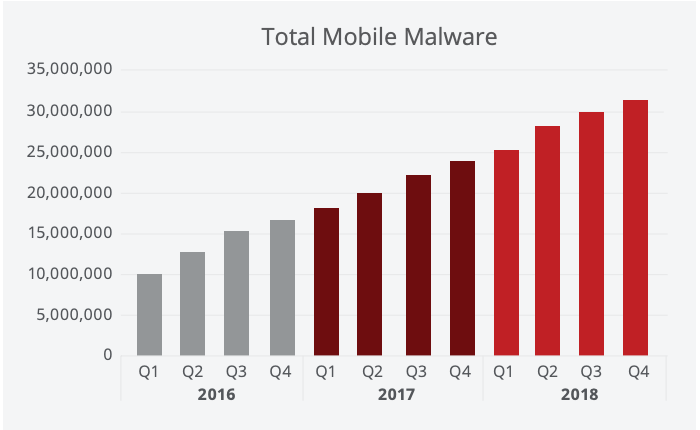
\includegraphics[scale=0.9]{./Figure/androidgraph.png}
    \caption{Total mobile malware \cite{mcafee}}
    \label{fig:androidgraph}
  \end{figure}

In order to mitigate the spread of malware, Google introduced a detection mechanism to its app market in Feb 2012 called Bouncer. Bouncer tests submitted applications in a sandbox for five minutes in order to detect any harmful behaviours; however, it has been shown that bouncer can be evaded by means of some simple detection avoidance methods. Alongside Bouncer, Google introduced Google Play protect in the Google 2017 event \cite{googleplay}. Google Play Protect is an always-on service that scans the applications automatically even after installation to ensure that the installed applications remains harmless 24/7. It has been reported that over 50 billion apps are scanned and verified every day regardless of where they were download from. However, according to McAfee, Google Play Protect also failed when tested against malware discovered in the previous 90 days in 2017 \cite{mcafee2018}. Furthermore, most third-party stores do not have the capability to scan and detect submitted harmful applications. Clearly, there is still a need for additional research into efficient methods to detect zero-day Android malware in the wild in order to overcome the aforementioned challenges.

Cyber attacks manage to produce unprecedented levels of disruption, where attackers usually leverage diverse tools and tactics, such as zero-day vulnerabilities and malware. This situation makes malware detection techniques worth studying and improving, in order to prevent and/or mitigate the effects of cyber attacks. Machine learning techniques can help to satisfy this demand,building classifiers that discern whether a precise Android application is malware or benignware. Algorithms such as Decision Trees, Support-Vector Machines and NaiveBayes, to name a few, are able to build such classifiers. Going further, ensemble methods for machine learning aim at effectively integrating many kinds of classification methods and learners to benefit from each ones advantages and overcome their individual drawbacks, hence improving the overall performance of the classification.

Various approaches have been proposed in previous works with the intention of detecting Android malware. These approaches are categorized into static analysis, dynamic analysis or hybrid analysis (where static and dynamic are used together). The methods based on static analysis reverse engineers the application for malicious code analysis. Arp et al. (2014) \cite{drebin}, M. Yusof et al \cite{apicallpaper}. Fan et al. (2017)\cite{dapasa}, are few examples of detection methods using static analysis. Static analysis of Android malware can rely on Java bytecode extracted by disassembling an application. The manifest file is also a source of information for static analysis. By contrast, dynamic analysis executes the application in a controlled environment such as an emulator, or a real device with the purpose of tracing its behavior. Several dynamic approaches, one of them is Alzaylaee, M.K., Yerima, S. Y., and Sezer S. (2016) DroidBox \cite{andropytool}. However, the efficiency of these approaches rely on the ability to detect the malicious behavior during the runtime while providing the perfect environment to kick-start the malicious code.
And many approaches do not have an end-to-end system to detect malware. They have some separated steps to predict and are not easy to use for users.

In this paper, we will focus on Static analysis methods to detect malware in \ac{apk} using features extracted from these \ac{apk} files with reverse engineering methods. We used a tool named AndroPytool\cite{andropytool} to extract 7 different Static features described at table\ref{table:1}. 


\begin{table}[htbp]
  \centering
  \caption{Static features used in our proposed system}
  \label{table:1}
  \begin{tabular}{|c||l l|}
  \hline
  & \textbf{Feature name} & \textbf{Description}\\
  \hline
  \multirow{7}{4em}{Static Feature}
   & API calls &  Count of system calls performed by an APK \\ 
   & Opcodes & Count of opcodes performed by an APK \\ 
   & Permissions & Which permissions uses the APK \\ 
   & Intent receivers & Set of an APK’s receivers \\ 
   & Intent services & Services used by an application \\
   & Intent activities & Activities declared by an APK \\ 
   & System commands & Set of system commands ran by the app \\ \hline
  
  \end{tabular}
  \end{table}

Using these features, we trained several machine learning models to predict if the application is a malware or not. Then we use these models predictions to train other new models to predict the malware application. This technique is called Stacking. It is a way to ensemble multiple classifications or regression models. This method is often used by data scientists in Kaggle \cite{kaggle} competitions to improve the final prediction and is one of the state-of-art techniques in table data competitions.
Furthermore, we propose an end-to-end system that uses for input an android \ac{apk} and output the result of detection, benign application or malware application. 

